\documentclass[11pt]{article}

\usepackage[utf8]{inputenc}
\usepackage[margin=1in]{geometry} 
\usepackage{amsfonts,amssymb,mathtools, amsmath, amsthm}

\usepackage{enumitem}
\usepackage{comment}
\usepackage{pbox}
\usepackage{float}

% drawing stuff
\usepackage{tikz}
\usepackage{tcolorbox}
\usepackage{pgf, tikz}
\usetikzlibrary{arrows, automata}

\usepackage{titling}

\usepackage{fancyhdr}
\usepackage{minted}
\usepackage[stable]{footmisc}

\usepackage{hyperref}
\hypersetup{
    colorlinks,
    citecolor=black,
    filecolor=black,
    linkcolor=black,
    urlcolor=black
}

\usepackage{booktabs, changepage}
\usepackage{parskip}
\usepackage{bold-extra}
\usepackage[ruled,vlined]{algorithm2e}
\DeclarePairedDelimiter\ceil{\lceil}{\rceil}
\DeclarePairedDelimiter\floor{\lfloor}{\rfloor}

\newcommand{\Z}{\mathbb{Z}}
\newcommand{\N}{\mathbb{N}}
\newcommand{\R}{\mathbb{R}}
\newcommand{\PS}{\mathcal{P}}
\newcommand{\bracket}[1]{\langle #1 \rangle}
\newcommand{\ttt}[1]{\texttt{#1}}


\newenvironment{ditem}[1][]
    {\begin{itemize}[label=--, topsep=-12pt,
    leftmargin = *, #1]
     \setlength\itemsep{0em}}
    {\end{itemize}}

\newcommand{\cbox}[2]{
    \centering{\fbox{\parbox{#1}{#2}} \par}
}

\newcommand{\contribBox}[2]{
{\centering{\fbox{\parbox{\textwidth}{\centering \textit{Collaborators}: #1 (Room #2)
}} \par}}
}

\floatname{algorithm}{Procedure}

\theoremstyle{definition}
\newtheorem{theorem}{Theorem}[section]
\newtheorem{exmp}{Example}[section]
\newtheorem{lemma}{Lemma}[section]


\newenvironment{mintedcpp}[0]
{%
  \VerbatimEnvironment
  \begin{minted}[
               mathescape,
               linenos,
               numbersep=5pt,
               gobble=2,
               frame=lines,
               framesep=2mm]{cpp}%
}
{%
  \end{minted}%
}

\setlength{\headheight}{14pt}
%\setlength{\parindent}{0pt}
%\setlength{\parskip}{6pt}

\newenvironment{shortsol}[0]
{%
    \textit{Solution}.
    \begin{adjustwidth}{2em}{2em}
}
{%
    \end{adjustwidth}
}

\pagestyle{fancy}
\fancyhead[L]{David Wen}
\fancyhead[C]{}
\fancyhead[R]{CSCI 270}

\begin{document}
\section{January 22, 2021}
\begin{exmp}
Every execution of the G-S algorithm (where men propose) results in the same stable matching regardless of the order in which men propose.
\end{exmp}
\begin{proof}
Prove that men obtain the best valid partner. For sake of contradiction, assume that the G-S algorithm will result in different stable matchings $S_1$ and $S_2$. Assume that in $S_1$ includes a pair in which a man does not have his best valid partner, meaning at least one rejection occured. Therefore, looking at the first time a man $m$ was rejected, he must have been rejected by his best valid partner $w$. Since $(m,w)$ is a valid pair, let $S_2$ include $(m,w)$. We know from the rejection that $w$ prefers some man $m'$ to $m$. Furthermore, because no man has been rejected yet and because men propose in order of preference, $m'$ prefers $w$ to the woman he is matched in $S_2$, say $w'$. Therefore, because $(m', w) \not \in S_2$, $S_2$ is not a stable matching, contradicting the claim that $S_2$ is stable.
\end{proof}
\begin{exmp}
Prove that when we run the G-S algorithm with men proposing, women end up with their worst possible partners.
\end{exmp}
\begin{proof}
Let $S*$ be a stable matching produced when men propose. Suppose that $(m,w) \in S*$, where $m$ is not the worst valid partner of $w$. Therefore, this implies that there is another stable matching $S$ where $(m', w), (m, w') \in S$. It follows from the previous problem that $m$ prefers $w$ to $w'$ in $S*$, and we assume in the premise that $w$ prefers $m$ to $m'$. Therefore, $(m',w)$ is an instability in $S$, contradicting that $S$ is stable.
\end{proof}
\begin{exmp}
Given $n$ men and $n$ women along with their preference lists, a \textbf{consensus-optimal stable matching} is a matching which simultaneously pairs every man with his best valid partner and pairs every woman with her best valid partner. Give an algorithm to determine whether a consensus-optimal stable matching exists for a given set of preference lists; the running time should be in \texttt{O($n^2$)} time.
\end{exmp}
\begin{proof}
Run the G-S algorithm with the men proposing once and the women proposing once. If $S_m = S_w$, then there is one single stable matching, since in $S_m$ the men are optimized, and in $S_w$ the women are optimized.
\end{proof}

\begin{exmp}
In every stable matching that G-S creates when men propose, it is possible that no man is matched to his highest rated woman.
\end{exmp}
\begin{proof}
Let the men's preferences be $m_1(w_1, w_3, w_2), m_2(w_1, w_2, w_3), m_3(w_3, w_1, w_2)$, and the women's preferences be $w_1(m_3, m_2, m_1), w_2(m_1, m_2, m_3), w_3(m_1, m_2, m_3)$. \\ The final pairings are $(m_1, w_3), (m_2, w_2), (m_3, w_1)$, where no man has their ideal matching.
\end{proof}
\newpage

\section{January 29, 2021}
\begin{exmp}
Arrange the following functions in increasing order of asymptotic growth rate.
\end{exmp}
\begin{enumerate}
    \item $f_6 = \log^2{n}$
    \item $f_5 = 2^{\log{n}} = n$
    \item $f_4 = n \log\log{n}$
    \item $f_1 = \log{n^n} = n \log n$
    \item $f_7 = n^{\sqrt{2}} \approx n \cdot n^{.4}$
    \item $f_2 = n^2 = n \cdot n$
    \item $f_3 = n^{\log{n}}$
\end{enumerate}
\begin{exmp}
Suppose $f(n), g(n)$ are two positive, monotonically increasing functions such that $f(n) = O(g(n))$. Is $2^{f(n)} = O(2^{g(n)})$?
\end{exmp}
False: let $f(n) = 2n, g(n) = n$. Then we see that $2^{f(n)} = 2^{2n} = 4^n$, which is not $O(2^{g(n)}) = O(2^n)$.

\begin{exmp}
Find an upper bound on the worst case runtime of the following code, assuming \texttt{find\_max} runs in linear time. Is it the tight upper bound?
\end{exmp}

\begin{verbatim}
    void func(int[] L, int n)
        while (n > 0)
            find_max(L,n);
            n = n/4;
\end{verbatim}
We have $f(n) = n + \frac{n}{4} + \frac{n}{16} + ... + \frac{n}{4^n}$. By the geometric series, this converges to $\Theta(n)$.

\begin{exmp}
Find a lower bound on the best case run time of the following code segment. Note that string concatenation is $O(n+m)$, NOT constant because it has to reallocate memory and copy over character-by-character. Is it the tight lower bound?
\end{exmp}
\begin{verbatim}
    string func2(int n)
        if (n == 0) return "a";
        string str = func2(n-1);
        return str + str;
\end{verbatim}
The tight lower bound is $\Theta(2^n)$, because it will run $n$ times, and on each iteration it will take $2^n$ operations.

\begin{exmp}
Erdos Number:
\begin{enumerate}
    \item Explain how to represent this data as a graph.
    \item Explain how we would compute the Erdos number for a particular researcher.
    \item Explain how we would determine all research with Erdos number at most two.
\end{enumerate}
\end{exmp}
\noindent\textbf{Solution:}
\begin{enumerate}
    \item Represent each researcher as a node and every co-authored paper as an edge.
    \item Do BFS from researcher $r$ to Erdos $e$.
    \item Do BFS from $e$, terminating once depth = 2.
\end{enumerate}
\begin{exmp}
Given a DAG, give a linear-time algorithm to determine if there is a simple path that visits all vertices.
\end{exmp}
First, create a topological sorting from the DAG. To do this, go through node by node and do DFS from each node; mark all visited nodes. When the DFS is finished, add the newly visited nodes to a stack in post-order traversal. Check if there's an edge from $n_i$ to $n_{i+1}, 1 \leq i \leq n-1$. 

\newpage
\section{February 5, 2021}
\begin{exmp}
In a connected bipartite graph, is the bipartition unique? What if it's not a connected bipartite graph? Explain.
\end{exmp}
Yes, prove by contradiction. let $G = (V,E)$ be the connected graph, and let $X \subset V$, $Y \subset V$ be the bipartition such that edges only exist between $X$ and $Y$. Assume there is another unique bipartition into $X', Y'$. Therefore, WLOG, $\exists x \in X'$ such that $x \in Y$. Then every edge connecting to $x$ must connect to a node $y \in Y'$. Extending this case, these nodes $y$ can connect only to nodes in $X'$, etc. Therefore, we have $X = Y'$ and $Y = X'$, so there cannot be another unique bipartition.

If it's not connected, then the bipartition is not necessarily unique. let's say we have nodes $\{A,B,C,D\}$ and edges $\{(A,B), (C,D)\}$. Then we can have $X = \{A,C\}$ and $Y = \{B,D\}$, and $X' = \{A, D\}$ and $Y' = \{B,C\}$.

\begin{exmp}
We want to drive from LA to SF in a car that stores enough gas to travel $p$ miles. We have a map with $n$ gas stations, such that there is distance $d_i$ between gas stations $g_i$ and $g_{i+1}$ along the route. Devise a greedy algorithm to minimize the stops, and prove that the solution is optimal. Give the time complexity of your algorithm as a function of $n$.
\end{exmp}

Let $p_i$ be the mileage of the car at gas station $i$. For every $i$, determine if $p_i < d_i$. If true, then stop at gas station $i$ and set $p_i$ to $p$. Repeat until the destination is reached.

\begin{proof}
\setlength{\parindent}{12pt}
Prove by induction. Let there exist an optimal solution with $k$ stops, such that $S = \{h_1, h_2, ..., h_k\}$. Assume our solution is optimal of size $m$, such that $S' = \{h_i', h_2', ..., h_k'\}$. Then we want to prove that every station that we stop in $S$, $h_i$, must come before or is the same as $h_i'$. \par
\textit{Base case:} $h_1 \leq h_1'$, since $h_1'$ is the last station that can be reached from the start without stopping.\par
\textit{Inductive hypothesis:} assume for $2 \leq i \leq k$, $h_k \leq h_k'$.\par
\textit{Inductive step:} Since the distance from $h_k'$ to $h_{k+1}'$ is less than or equal to the distance from $h_k$ to $h_{k+1}'$, we can easily see that our solution is the same as or ahead of the other optimal solution. \\[1em]
The time complexity is O($n$), since we only do one computation at each gas station.
\end{proof}

\begin{exmp}
Imagine you are a CP for a CSCI 270 discussion section. You have $n$ problem categories to work through. Each problem category has a learning value of $I_i$ per question and a completion time of $t_i$ per question. However, you only have $K$ minutes per discussion. Find a greedy algorithm to determine which problems to complete to maximize the learning value. You can also do a portion of the problem.
\end{exmp}
The algorithm is to sort the problems in decreasing ration of learning value, $x_i$ = $\frac{l_i}{t_i}$. Then select the problems in order, and do as much as the last problem. The proof is the same as before: basically at every step, the cumulative sum of $x$ is better or the same as another optimal solution, since we choose the values that have the highest $x_i$.

\begin{exmp}
You organize a triathlon "relay" with three athletes, each who ha a projected swimming, biking, and running time, but you have a one lane pool (i.e. only one person can swim at a time). You want to schedule athletes such that all three athletes can finish in the minimum amount of total time.
\end{exmp}
Let us order the athletes $x_1, x_2, x_3$ in order of descending land sport completion time. The time taken will be \texttt{max(a1+b1, a1+a2+b2, a1+a2+a3+b3)}, where $a$ is the swimming time and $b$ is the land time. Prove that this is the best order by exchange argument.

\begin{exmp}
We have a collection of stones, each with a positive integer weight. Each turn we choose the two heaviest stones and smash them. Suppose the stones have weight $x$ and $y$, $x \leq y$. Then if $x = y$, both are destroyed, and if $x \neq y$, x is destroyed, and the stone weight has new weight $y-x$. Give an algorithm to give the weight of the last stone (if there is one).
\end{exmp}
Algorithm:
\begin{enumerate}
    \item Initialize a \textbf{max-heap} of integers.
    \item Construct the heap with weights.
    \item Then iterate:
    \begin{verbatim}
    while size(heap) > 1:
        max1 = heap.pop()
        max2 = heap.pop()
        if max1-max2 > 0: 
            heap.push(max1-max2)
    if size(heap) == 1:
        return heap.top()
    if size(heap) == 0:
        return 0
    \end{verbatim}
\end{enumerate}
The time complexity is O($n \log n$). We can construct the heap in O($n$) time, we have at most $n$ iterations in the loop (we remove at least 1 stone each iteration), and we have 3 O($\log n$) operations in the loop (remove, remove, add). The space complexity is O($n$), though if you're allowed to modify the input array it can be done without any additional space.

\begin{exmp}
Find the $k^{th}$ largest element in an unsorted array.
\end{exmp}
A naive solution is to sort the array in descending order, then output the $k^{th}$ element. This takes O(n $\log n$).

A better solution with runtime O($n \log k$), space of $k$:
\begin{enumerate}
    \item Initialize a min-heap
    \item Add elements into the heap, and pop when the size of the heap grows above $k$.
    \item Pop the top (min) once everything is done.
\end{enumerate}

\newpage
\section{February 12, 2021}
\begin{exmp}
    Let $e^*$ be the cheapest edge in an undirected graph. Answer true or false: 
    \begin{enumerate}
        \item If edge costs are distinct, there is a MST containing $e^*$. \textbf{True}.
        \item If edge costs are all distinct, all MSTs contain $e^*$. \textbf{True}.
        \item There is always a MST containing $e^*$. \textbf{True}.
        \item All MSTs contain $e^*$. \textbf{False.}
    \end{enumerate}
\end{exmp}
\begin{exmp}
    Suppose you are given a connected graph $G$ with edge costs that are all distinct. Prove that $G$ has a unique minimum spanning tree.
\end{exmp}
    Suppose there is more than one unique MST, $T$ and $T'$. Therefore, there must be some edge $e \in T, e \not\in T'$. When $e$ is added to $T'$, then a cycle is formed. Then remove the edge with the highest cost in the cycle formed in $T'$. If $e$ is removed, then $T'$ has a lower total cost than $T$, so $T$ is not an MST. Otherwise, if $e$ is not removed, then we have lowered the cost of $T'$, meaning $T$ was not a MST. Therefore, one of these trees are not a MST.
    
\begin{exmp}
    Recall that Dijkstra's requiers edge weights to be non-negative. Suppose the minimum-weight edge in the graph has weight $-w$. If we add $w+1$ to every edge, does Dijkstra's find the original shortest path?
\end{exmp}
No it does not. Take the following simple example where we have $A\rightarrow B$ is -7, $B\rightarrow C$ is 10, and $A \rightarrow C$ is 4. The shortest path is to go $A \rightarrow B \rightarrow C$. However, by adding 8 to all nodes, the shortest distance becomes 12, by $A \rightarrow C$.

\begin{figure}[H]
    \centering
    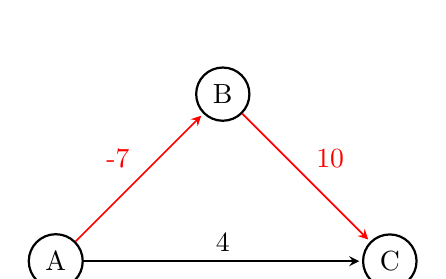
\begin{tikzpicture}[
            > = stealth, % arrow head style
            shorten > = 1pt, % don't touch arrow head to node
            auto,
            node distance = 3cm, % distance between nodes
            semithick % line style
        ]
        \tikzstyle{every state}=[
            draw = black,
            thick,
            fill = white,
            minimum size = 4mm
        ]
        \node[state] (A) {A};
        \node[state] (B)[above right of=A] {B};
        \node[state] (C)[below right of=B] {C};
        
        \path[->, red] (A) edge node{-7} (B);
        \path[->] (A) edge node{4} (C);
        \path[->, red] (B) edge node{10} (C);
    \end{tikzpicture}
    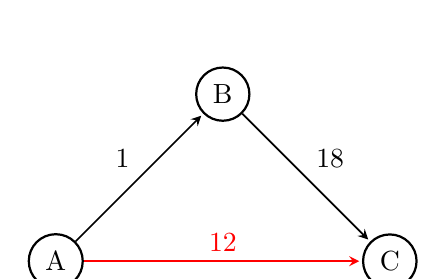
\begin{tikzpicture}[
            > = stealth, % arrow head style
            shorten > = 1pt, % don't touch arrow head to node
            auto,
            node distance = 3cm, % distance between nodes
            semithick % line style
        ]
        \tikzstyle{every state}=[
            draw = black,
            thick,
            fill = white,
            minimum size = 4mm
        ]
        \node[state] (A) {A};
        \node[state] (B)[above right of=A] {B};
        \node[state] (C)[below right of=B] {C};
        
        \path[->] (A) edge node{1} (B);
        \path[->, red] (A) edge node{12} (C);
        \path[->] (B) edge node{18} (C);
    \end{tikzpicture}
\end{figure}

Note: if we add $c$ to every edge in a graph, the MST will remain the same because every MST will contain $n-1$ edges, and the relative edge weights do not change.
\begin{exmp}
    \begin{enumerate}
        \item Explain how to implement a FIFO queue with 2 stacks. Show how to implement enqueue and dequeue.
        \item Show enqueue runs in constant time and dequeue runs in amortized constant time.
    \end{enumerate}
\end{exmp}
Let us define two stacks $A$ and $B$. To enqueue, simply push to stack $A$. To pop, If $B$ is empty, while $A$ is not empty, pop $A_i$ from $A$ and push $A_i$ onto $B$. Then pop from $B$. 

Enqueue runs in constant time because it just uses the stack push operation, which runs in constant time.

Dequeue accounting analysis:
Let the credit of push be 2, pop be 0, and "flip" be 1. If we do $n$ pushes, we have a credit of $2n$. Then when we do one pop, we do a "flip:" $n$ pops from $A$ and $n$ pushes to $B$. Thus, we have a credit of 0 after this one pop. We see that the currency never drops below 0, so these operations are amortized constant time.

\newpage
\section{February 17 -- Lecture Review}
\begin{exmp}
    \textbf{Klein and Tardos, Chapter 1, 6 and 7}.
\end{exmp}
We want to avoid the case where ship $s$ stops at port $p$ on day $d$, but $s'$ would visit on some $d' > d$. Treat this problem in the same way as a stable matching problem: each port $p$ ranks ships in reverse chronological order (want to see as many ships as possible), and each ship ranks ports in chronological order (want to stop ASAP).
\begin{exmp}
    \textbf{Asymptotic Notation:} rank the following: $4^nn^4, \log_2{n}, 2^{\sqrt{\log n}}, 2^n, 2^nn^8, \log_4{n},$, $\sqrt{n}, n^{\log n}$.
\end{exmp}
\textit{Ranking}: $\log_2{n} = \log_4{n} < 2^{\sqrt{\log n}} < \sqrt{n} < n^{\log n} <  2^n <  2^nn^8 < 4^nn^4$

\begin{exmp}
    \textbf{DFS vs. BFS}. 
    \begin{itemize}
        \item If $e \in G$ but not in the BFST, then $e$ must be between \textit{nodes on the same or consecutive layers of the BFST}.
        \item If $e \in G$ but not in the DFST, then $e$ must be between \textit{a node and its ancestor}.
    \end{itemize}
    \textbf{Solve the following}:
    \begin{enumerate}
        \item Find the shortest path: \textit{BFS}.
        \item Find a cycle: \textit{BFS or DFS}.
        \item Find an odd-length cycle: \textit{BFS or DFS} (recall: bipartite graphs).
    \end{enumerate}
\end{exmp}

\begin{exmp}
    A pharmacist has $W$ pills and $n$ empty bottles. Let $P = \{p_1, p_2, ..., p_n \}$ denote the number of pills that each bottle can hold. Describe a greedy algorithm, which, given $W$ and $\{p_1, p_2, ..., p_n\}$ determines the fewest number of bottles needed to store the pills. Prove the correctness.
\end{exmp}
\textit{Solution}: sort $P$ in descending capacity. Fill the largest emptiest bottle, then repeat while there are pills to be bottled.

\begin{proof}
Assume that our algorithm produces a solution $A$, and there is another optimal solution $O$, such that $|A| = |O|$. Prove by induction that our solution stays ahead:
\begin{adjustwidth}{2em}{2em}
\textit{Base case:} $i = 1$. We fill the biggest bottle, so we have filled the most pills positive with one bottle. \par
\textit{Inductive case:} Assume that our algorithm stays ahead on bottle $k$. Since we have filled the most pills possible with $k$ bottles, and we pick the next-largest bottle, we still must have filled as many bottles with $k+1$ bottles, so we must have stayed ahead of, or is the same as $O$.
\end{adjustwidth}
\end{proof}

\begin{exmp}
    You are given two lists of positive integers, $A$ and $B$, such that $|A| = |B| = N$. You may rearrange the elements of each list however you like. Then compute:
    $$ \prod_{i=0}^N a_i^{b_i} $$
    Our goal is to maximize this product. Provide an algorithm such that this product is maximized.
\end{exmp}
\textit{Solution:} Sort both lists $A$ and $B$ in descending order.
\begin{proof}
Prove by exchange argument. Assume there is some optimal solution $O$ with $k$ inversions. Without loss of generality, let's say elements $b_i, b_j$ have been inverted, such that $i < j$. Then in our solution, we have $a_i \leq a_j$, $b_i \leq a_j$. Then in $O$, our cost changes by:
\begin{align*}
    \frac{C_A}{C_O} &= \frac{a_i^{b_i}a_j^{b_j}}{a_i{^{b_j}} a_j^{b_i}} \\
    &=  a_i^{b_i-b_j}a_j^{b_j-b_i} \\
    &=  \frac{a_j^{b_j-b_i}}{a_i^{b_j-b_i}} \\
    &\geq 1
\end{align*}
\end{proof}
\begin{exmp}
    \textbf{Heaps.} Given an array $A$ of $n$ numbers and for an integer $k \leq n$, what is the time complexity of extracting the $k$ smallest numbers in the array? $O(n + k\log n)$. It costs $n$ to construct the heap, and $k \log n$ to extract.
\end{exmp}

\begin{exmp}
    \textbf{MST Problems.} It's the homework questions about MSTs and minimum bottleneck spanning trees. Yay
\end{exmp}

\begin{exmp}
\begin{itemize}
    \item Given a weighted undirected graph $G$, adding weight $k$ to every edge, resulting in graph $G'$, will allow Dijkstra's algorithm to find the same solution in both $G$ and $G'$. \textit{False}.
    \item Given a weighted undirected graph $G$, multiplying each edge weight by $k$, resulting in graph $G'$, will allow Dijkstra's algorithm to find the same solution in both $G$ and $G'$. \textit{True}.

\end{itemize}
\end{exmp}

\newpage
\section{February 26, 2021}
\begin{exmp}
Solve the following by the Master's theorem:
\begin{enumerate}
    \item $T(n) = 9T(\frac{n}{3}) + n + \log n$
    \item $T(n) = 4T(\frac{n}{2}) + n^3$
    \item $T(n) = 4T(\frac{n}{2}) + n^2$
    \item $T(n) = 4T(\frac{n}{2}) + n$
\end{enumerate}
\end{exmp}
\textit{Solution}.
\begin{enumerate}
    \item We have $a = 9, b = 3$, so $n^{\log_b{a}} = n^2$. Our $f(n) = n \log n$, so this function falls under case 1. Therefore, $T(n) = \Theta(n^2)$.
    \item We have $a = 4, b = 2$, so $n^{\log_b{a}} = n^2$. Our $f(n) = n^3$, so this function falls under case 3. We also have the verify that $a f(\frac{n}{2}) \leq cf(n)$, which is $4 \frac{n^3}{8} \leq cn^3$, which works for $c = 1$. Therefore, $T(n) = \Theta(n^3)$.
    \item We have $a = 4, b = 2$, so again $n^2$. Since $f(n) = n^2$, this falls under the case 2. so $T(n) = n^2\log{n}$.
    \item We have $a = 4, b = 2$, so again $n^2$. Since $f(n) = n$, this falls under case 1, so $T(n) = \Theta(n^2)$.
\end{enumerate}
\begin{exmp}
Suppose you have two sorted arrays $A$ and $B$ of size $n$ each. Design a divide and conquer algorithm to find the median of the array obtained after merging the two arrays. Find the runtime complexity.
\end{exmp}
\textit{Solution}:

\begin{algorithm}[H]
\caption{find\_median(A,B,n)}
m\_a = median of A\;
m\_b = median of B\;
\If{m\_a = m\_b}
{
    return m\_a\;
}
\ElseIf{m\_a < m\_b}
{
    A' = right half of A\;
    B' = left half of B\;
    return find\_median(A', B')\;
}
\ElseIf{m\_b < m\_a}
{
    A' = left half of A\;
    B' = right half of B\;
    return find\_median(A', B')\;
}
\end{algorithm}
The runtime $T(n) = aT(\frac{n}{b}) + f(n)$. Since we are discarding half the problem at each step, and it remains one problem, we get $a = 1, b = 2$. $f(n) = O(1)$ since it is constant work at the root, and $\log_b{a} = 0$. Therefore, this falls under case 2, so $T(n) = \Theta(\log(n))$. Because this code is recursive, this code takes $\log(n)$ space, but it can be done iteratively in place.

\begin{exmp}
We have a sorted array of distinct integers $A$, and we want to decide if there is an index $i$ for which \texttt{A[i] = i} (i.e. \textbf{fixed point}). Describe an efficient divide-and-conquer algorithm that solves this problem and explain the time complexity.
\end{exmp}
\begin{algorithm}
\caption{find\_index(A, s, f)}
\If{s $<$ f}{return -1\;}
i = (s+f)/2\;
\If{A[i] = i}{return i\;}
\If{A[i] $<$ i}{return find\_index(A, i+1, f)}
\ElseIf{A[i] $>$ i}{return find\_index(A, s, i-1)}
\end{algorithm}
This is basically just binary search, which no one has ever implemented correctly on the first attempt. The runtime is $\Theta(\log n)$ as before.
\begin{exmp}
Let $f(x)$ be a continuous function such that $f(x): \lbrack 0, 1 \rbrack \rightarrow \lbrack 0, 1\rbrack$. Find or approximate $x$ such that $f(x) = x$.
\end{exmp}
\begin{algorithm}
\caption{Find fixed point of a function $f(x)$.}
\If{f(0) = 0}{return 0\;}
\If{f(1) = 1}{return 1\;}
l = 0\;
r = 1\;
\While{r - l $>$ precision}
{
    m = (l+r)/2\;
    \If{f(m) = m}{return x = m\;}
    \ElseIf{f(m) $>$ m}{l = m\;}
    \ElseIf{f(m) $<$ m}{r = m\;}
}
\end{algorithm}
\begin{exmp}
A \textit{tromino} is a figure composed of three 1x1 squares in the shape of an L (i.e. a $2 \times 2$ square missing a square). Given an $2^n \times 2^n$ checkboard with 1 missing square, tile it with trominoes. 
\end{exmp}
Split the squares
\end{document}
